% ----------------------------------------------------------
% Teste test3_4_e25b32class2_20231211_234707
% ----------------------------------------------------------
\subsubsection{Teste test3_4_e25b32class2_20231211_234707 - AlexNet (Is That a Santa)}

Informações utilizadas para o treinamento.

\begin{table}[ht]
   \centering
   \caption{Treinamento}
   \label{tab:modelos}
   \begin{tabular}{| c | c | }
      \hline 
      \textbf{Informação} & \textbf{Descrição} \\
      \hline \hline 
      Rede & AlexNet \\
      \hline
      Número de épocas & 25\\
      \hline
      Tamanho do lote & 32\\
      \hline
      Taxa inicial & 0.012 \\
      \hline
      Taxa de decaimento & 0.0006 \\
      \hline
      Total de classes & 2\\
      \hline
      Dataset & CIFAR-10\\
      \hline
   \end{tabular} 
\end{table}

Resultados obtidos após treinamento.

\begin{tabular}{lrrrr}
\toprule
  Unnamed: 0 &  precision &  recall &  f1-score &  support \\
\midrule
       Santa &       0.50 &     1.0 &  0.666667 &    307.0 \\
   Not Santa &       0.00 &     0.0 &  0.000000 &    307.0 \\
    accuracy &       0.50 &     0.5 &  0.500000 &      0.5 \\
   macro avg &       0.25 &     0.5 &  0.333333 &    614.0 \\
weighted avg &       0.25 &     0.5 &  0.333333 &    614.0 \\
\bottomrule
\end{tabular}


\begin{figure}[ht]
 \begin{center}
   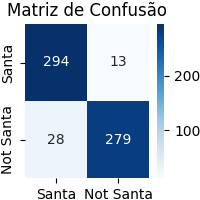
\includegraphics[scale=1]{tests/test3_4_e25b32class2_20231211_234707/confusion_matrix.png}
  \caption{Matriz de Confusão}
  \label{fig:fig03}
 \end{center}
\end{figure}

\begin{figure}[ht]
 \begin{center}
   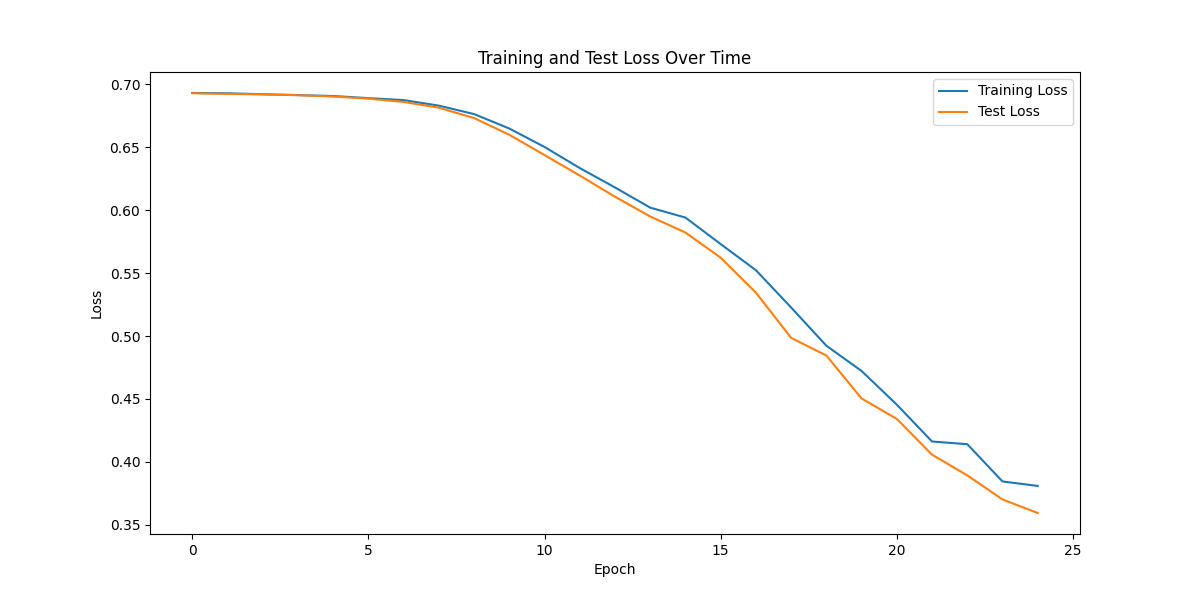
\includegraphics[scale=0.8]{tests/test3_4_e25b32class2_20231211_234707/loss_over_time.png}
  \caption{Gráfico de Perda}
  \label{fig:fig04}
 \end{center}
\end{figure}
